\section{temperature measurement}
\label{sec:tempmeas}
We  describe  here  some  details  on  the  analysis  to  measure  the
temperature with the  sun flux. This analysis is  being carried out by
Corinne in Grenoble  and Romain in Paris. \\ The basic  idea is to use
the  monitoring data to  measure the  raise of  the baseline  upon the
passage of  the sun in the  field of view of  GIGADuck's antenna. This
raise  is used  to  estimate  the noise  temperature  of the  GIGADuck
system. The main steps of the analysis are:


\begin{figure}[!ht]
 \centering
 \hspace*{-3ex}
 \subfigure{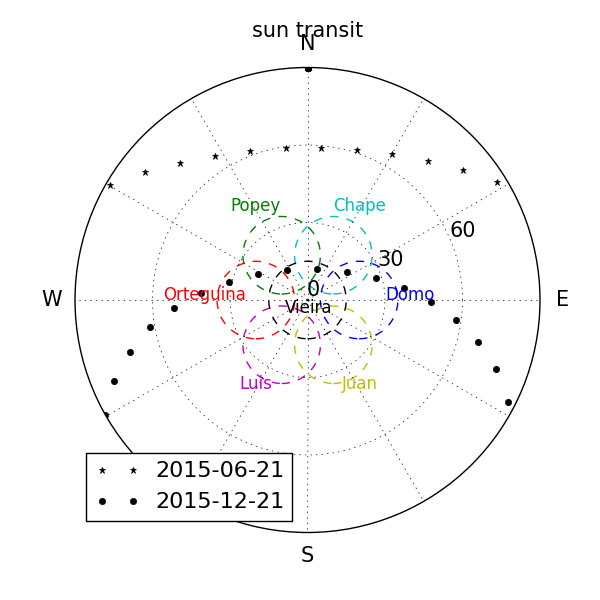
\includegraphics[width=0.49\linewidth]{sunpolar.png}}
 \subfigure{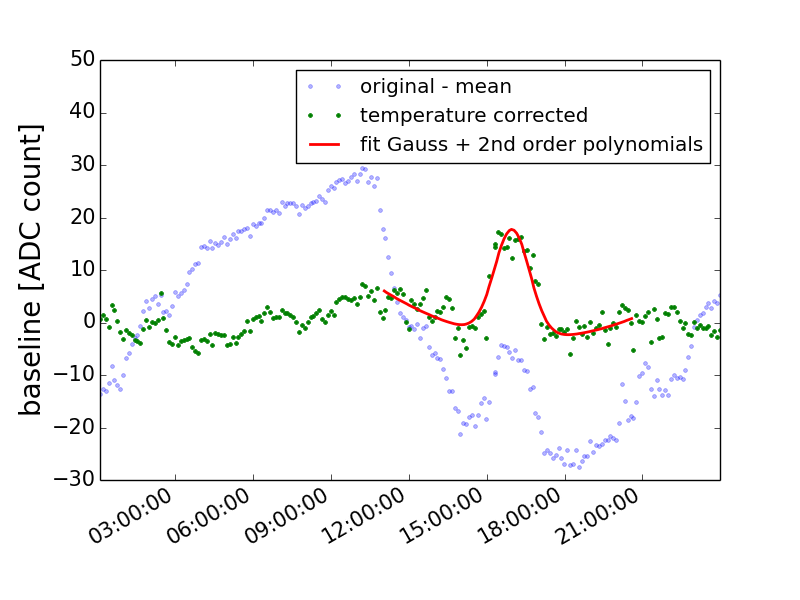
\includegraphics[width=0.49\linewidth]{examplesunfit.png}}
%% \subfigure{\includegraphics[width=0.49\linewidth]{sunexpected.png}}
 \caption{Left: Sun transit for the two solstices. The colored circles
   represent  the field  of  view of  the  GIGADuck antennas.   Right:
   Example  of the  baseline during  one  day. In  blue is  the
   orignal baseline when the mean is subtracted, in green after it was
   corrected from temperature dependence and  in red is a gaussian fit
   of to extract the signal from the sun.}
%%    Simulated  baseline  increase for  three  antennas  during the  sun
%%    passage.}
 \label{fig:sunsim}
\end{figure}


\begin{itemize}
\item produce the monitoring data
\item choose a period when the expected sun signal is large
\item cut the rainy periods
\item  find the  dependence of  the  radio baseline  with the  outside
  temperature during this period
\item correct the baseline for the outside temperature dependence
\item  fit the  radio baseline  with a  Gaussian plus  a  second order
  polynomial.
\end{itemize}




The figure~\ref{fig:sunsim} (left)  shows the path of the  sun for two
different dates and the field of  view of the GD C-band antennas.  The
sun signal  will be maximum  in summer when  the sun is higher  in the
sky.   The plot on  the right  in the  figure~\ref{fig:sunsim} (right)
shows the raw baseline of one antenna during one day in blue, the same
baseline corrected by  the tempereature dependence and the  fit of the
sun  bump in  red.  In  Corinne's  analysis, the  fit is  done with  a
constant  instead of  a  polynomials and  it  is done  on the  several
(around three)  consecutive days.  \\The  two methods have  shown very
similar  results.  They  show  differences between  antennas but  also
differences for  the same  antenna at different  time of the  year. We
intend in the next section  of this note to estimate the uncertainties
on this measurement to quantify the consistency of these results. 





